\subsubsection{Move computation to data, not vice versa}
\label{sec:technology:data_to_computation}

\LB придерживается следующего принципа: "Move com\-pu\-ta\-tion to data, not vice versa". Это достигается с помощью двух составляющих:

\begin{enumerate}
  \item dataflow graph (граф потока данных);
  \item incremental view maintenance (поэтапное поддержание представлений)
\end{enumerate}

Идея \emph{dataflow graph} (рисунок \ref{fig:technology:data_to_computation:dataflow_graph}) была использована в 1980-90 гг. в оптимизации компиляторов. Представление программы в виде такого графа вместо ее императивной структуры (сверху-вниз и слева-направо) позволяет автоматически ее параллелить. Например, для простой программы следующего вида можно составить граф, представленный на рисунке \ref{fig:technology:data_to_computation:dataflow_graph_parallel}, на котором также можно выделены операции, которые можно запустить параллельно (разные ветви графа):

\begin{lstlisting}[language=Pascal]
x := a * b;
y := 5 + x;
z := c + a;
\end{lstlisting}

\begin{figure}
	\centering
	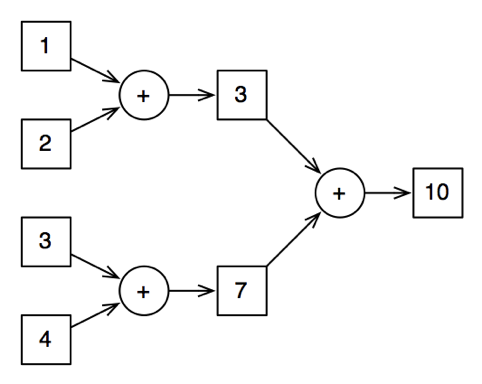
\includegraphics[scale=0.9]{dataflow_graph.png}
	\caption{Пример графа потока данных}
	\label{fig:technology:data_to_computation:dataflow_graph}
\end{figure}

\begin{figure}
	\centering
	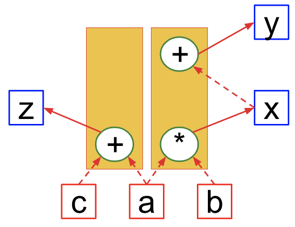
\includegraphics[scale=1.0]{dataflow_graph_parallel.png}
	\caption{Пример возможности параллелизации программы с помощью графа потока данных}
	\label{fig:technology:data_to_computation:dataflow_graph_parallel}
\end{figure}

Если же в примере заменить операцию присвоения на символ стрелки (\lstinline{<-}), то получится костяк программы на \logiql:

\begin{lstlisting}[language=Prolog]
x <- a * b.
y <- 5 + x.
z <- c + a.
\end{lstlisting}

Язык создан таким образом, чтобы среда выполнения могла построить такой dataflow graph. Затем по такому графу выполняется \emph{incre\-men\-tal view maintenance}. Он нужен для того, чтобы уменьшить количество пересчитываемых данных, в этом также помогает уже построенный dataflow graph. К примеру, из приведенного фрагмента программы (на рисунке \ref{fig:technology:data_to_computation:dataflow_graph}) можно понять, что при обновлении переменной \lstinline{c} необходимо лишь пересчитать значение переменной \lstinline{z}, а если поменялось значение \lstinline{a}, тогда нужно провести вычисления для всех переменных (\lstinline{x}, \lstinline{y}, \lstinline{z}).

Кроме того, в некоторых случаях даже обновление переменных не требует пересчета всей ее формулы. Например, в случае суммы \lstinline{a := x + y + z} изменение одного аргумента (\lstinline{y}) влечет лишь обычное изменение целевой переменной \lstinline{a} без дополнительного знания значений остальных аргументов (\lstinline{x} и \lstinline{z}).

Что же со всем этим делает платформа? На самом деле, \emph{вершины-данные} представляются как предикаты (аналог таблиц в \sql), а \emph{вершины-функции} - это запросы или вызовы оптимизационных решателей. Дальнейшее использование такого представления не вызывает лишних вопросов.
